% TODO Wishlist of things to cover
% Wikipedia as source for equations
% Things that suck in latex


\documentclass{beamer}
%
% Choose how your presentation looks.
%
% For more themes, color themes and font themes, see:
% http://deic.uab.es/~iblanes/beamer_gallery/index_by_theme.html
%

% Theme License: https://creativecommons.org/licenses/by/4.0/

\mode<presentation>
{
  \usetheme{metropolis}   % https://github.com/matze/mtheme
  \usecolortheme{default} % or try albatross, beaver, crane, ...
  \usefonttheme{default}  % or try serif, structurebold, ...
  \setbeamertemplate{navigation symbols}{}
  %% \setbeamertemplate{caption}[numbered]
  \setbeamertemplate{caption}{\raggedright\insertcaption\par}
}

\usepackage[english]{babel}
\usepackage[utf8x]{inputenc}
\PassOptionsToPackage{hyphens}{url}\usepackage{hyperref}

\title{An Introduction to \LaTeX}
\author{Jake Vossen}
\institute{Colorado School of Mines - acm-w}
\date{2020-02-26}

\begin{document}
\begin{frame}{Something to consider...}
    \begin{figure}
    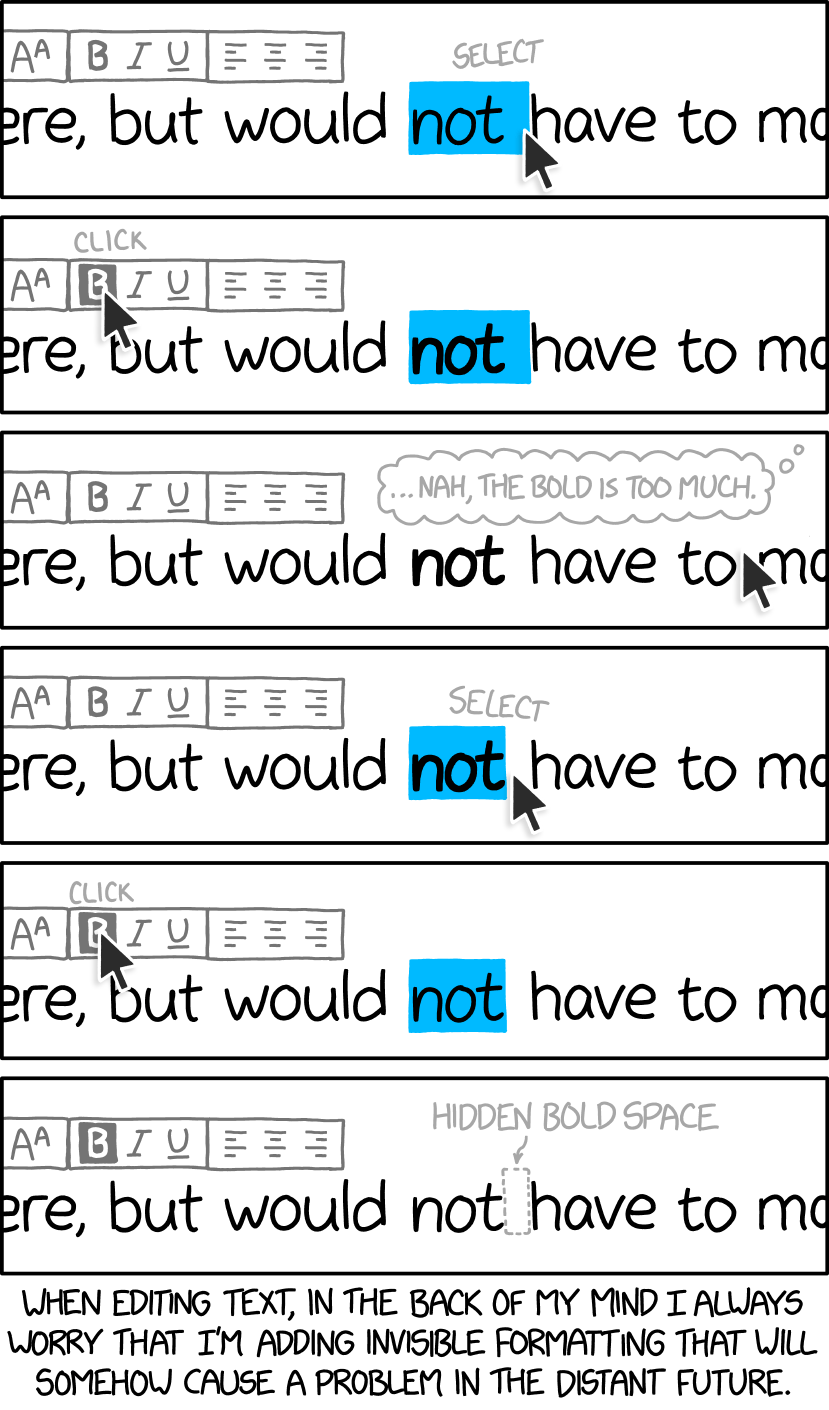
\includegraphics[scale=.13]{invisible_formatting_2x.png}
    \caption{https://xkcd.com/2109/}
  \end{figure}
\end{frame}
\begin{frame}
  \titlepage
\end{frame}

% Uncomment these lines for an automatically generated outline.
%\begin{frame}{Outline}
%  \tableofcontents
%\end{frame}

\section{What is \LaTeX?}

\begin{frame}[fragile]
  \frametitle{What is \LaTeX}

  It is \textbf{not} a ``what you see is what you get'' editor (WYSIWYG). \LaTeX converts plain text files (.tex) into (typically) PDFs

  %% text
\begin{verbatim}
  \begin{equation}
        x = \frac{ - b \pm \sqrt{b^2 - 4 a c}}{2a}
  \end{equation}
\end{verbatim}
\par
  \hrulefill\par
%% \hline
  \begin{equation}
        x = \frac{ - b \pm \sqrt{b^2 - 4 a c}}{2a}
  \end{equation}

\end{frame}

\begin{frame}[fragile]
\frametitle{More \LaTeX}
\begin{verbatim}
\begin{equation}
  \int_0^a x^n dx = \frac{1}{n+1}\
  a^{n+1} \qquad n \geq 0
\end{equation}
\end{verbatim}\par
  \hrulefill\par

\begin{equation}
  \int_0^a x^n dx = \frac{1}{n+1}\
  a^{n+1} \qquad n \geq 0
\end{equation}

\end{frame}

\section{The Why}


\begin{frame}[fragile]
  \frametitle{Widespread use in Academia}

  \begin{enumerate}
    \item {Almost all journals, especially in Math, CS, and Physics
      either prefer or mandate \LaTeX as the document submission
      format}
    \item {Discrete Math (CSCI 358) uses \LaTeX for all of your homework}
    \item {It can make your project / homework submissions look much more professional}
   \end{enumerate}

\vskip 1cm

\end{frame}

\begin{frame}[fragile]
  \frametitle{Better looking equations (arguably)}

  \begin{itemize}

  \item{Word}

  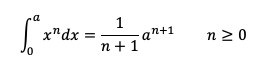
\includegraphics[scale=.75]{word-equation.png}

  \item{\LaTeX}

  \begin{equation}
  \int_0^a x^n dx = \frac{1}{n+1}\
  a^{n+1} \qquad n \geq 0
  \end{equation}

  \end{itemize}

\end{frame}

\begin{frame}{Quality of Life}
  \begin{itemize}
    \item {Use your favorite text editor to write those long papers}
    \item {Use git to version control and collaborate on writeups}
    \item {More control over how your document is formatted without having drag everything to how you like it}
    \item {A better ``default'' look instead of just bolding headings}
  \end{itemize}
\end{frame}

\begin{frame}[fragile]

  \frametitle{``Hello World'' document}
  \begingroup
  \fontsize{8pt}{10pt}\selectfont
  \begin{verbatim}
    \documentclass{article}
    \usepackage[margin=1in]{geometry}
    \begin{document}
    
    \title{Title Here}
    \author{Jacob Vossen}
    \maketitle
    \begin{abstract}
    The abstract text goes here.
    \end{abstract}
    \section{Introduction}
    Here is the text of your introduction.
    \subsection{Subsection Heading Here}
    Write your subsection text here.
    \section{Conclusion}
    Write your conclusion here.
    
    \end{document}
  \end{verbatim}
\endgroup
\end{frame}

\begin{frame}
  \begin{itemize}
    \item This slide exists to remind Jake to show you the example Hello World document
  \end{itemize}
\end{frame}
  

\section{Parts of a \LaTeX document}

\begin{frame}[fragile]
  \frametitle{The Header}
  \begin{verbatim}
  \documentclass{article}
  \usepackage[margin=1in]{geometry}
  \begin{document}
  \end{verbatim}

  \begin{itemize}
    \item{Document class - typically \texttt{article}, but you would change this if you where working on a book or thesis (or slides like these)}
    \item {Packages - easiest way to extend \LaTeX to include more functionality (in this case, setting margins away from the default 2 inches)}
  \end{itemize}
\end{frame}

\begin{frame}[fragile]
  \frametitle{The Title}
  \begin{verbatim}
   \title{Title Here}
   \author{Jacob Vossen}
   \maketitle
  \end{verbatim}

  \begin{itemize}
    \item {Title is automatically created and formatted with \texttt{\\maketitle}}
  \end{itemize}
\end{frame}

\begin{frame}[fragile]
  \frametitle{The Body}

  \begin{verbatim}
    \section{Introduction}
    Here is the text of your introduction.
    \subsection{Subsection Heading Here}
    Write your subsection text here.

  \end{verbatim}
% TODO Add verbatim to the subsection texts
  This is the meat of writing \LaTeX documents, using section, subsection, and subsubsection etc to structure your document, adding in equations when you need them. 


\end{frame}

\begin{frame}{Examples}
  \begin{itemize}
  \item{If you didn't guess already, these slides are in \LaTeX ! You can find them at \url{https://github.com/jakevossen5/acm-w-latex-talk}}
  \item {Some other examples...}
  \end{itemize}
  
\end{frame}


\begin{frame}{How to get Started with \LaTeX}
  In approvement order of most tech-intensive to least tech-intensive
  \begin{enumerate}
    \item{Overleaf - The Google Docs equivelent of \LaTeX - everything is in browser}
    \item { $\langle \text{Texpad, Texstudio, Texmaker} \rangle$ are all desktop apps designed for out of the box \LaTeX usage}
    \item {Using pdflatex (on macOS: brew cask install mactex) + the text editor of your choice} %TODO verb
  \end{enumerate}
\end{frame}


\begin{frame}{Things That Suck in \LaTeX}

  \begin{itemize}
    \item {The error messages are not the best, usually point to something quite a ways after what is actually wrong}
    \item {You have to rely almost entirely on third party documentation (Overleaf)}
    \item {Making tables can be a pain}
    \item {Adding diagrams exactly where you want them is difficult as well}
    \item {It can be frustrating when your English homework doesn't compile}
  \end{itemize}

  % Git, text editors, etc
\end{frame}

\begin{frame}{Getting Help on \LaTeX}
  Official documentation is not great, try the following places for good documentation / tutorials

  \begin{enumerate}
    \item<1->{\url{overleaf.com/learn} provides a \textbf{ton} of information on getting started with \LaTeX}
    \item<2-> {\url{tex.stackexchange.com}}
    \item<3-> {Wikipedia equations are all written in \LaTeX, if you have a specific equation or aren't sure how to do something}
    \item<4-> {Google - you are a comp sci after all}
  \end{enumerate}
\end{frame}

\begin{frame}{Personal Suggestions}
  \begin{enumerate}
    \item<1-> {VSCode + \LaTeX workshop for good side by side editing}
    \item<2-> {Keep a note file somewhere with all the header items you want to have in all of your documents}
    \item<3-> {Be willing to put some upfront cost in for long term benefit - it can be a bit of a frustrating experience to start but a rewarding one if you commit to it.}
    \item<4-> {Use git!}
  \end{enumerate}
\end{frame}



\end{document}
